%% AstroVista Lite: an arXiv manuscript (astro-ph.IM).  Build with `make` in this folder;
%% the figures and numbers come from ../make_figures.py.
\documentclass[twocolumn]{aastex701}

\usepackage{amsmath}

\newcommand{\avl}{AstroVista Lite}
\newcommand{\code}[1]{\texttt{#1}}

\begin{document}

\title{AstroVista Lite: Isophote Fitting, Source Finding and Masks for Astronomical
Images in One Window}

\author[0000-0002-5514-3354]{Ehsan Kourkchi}
\affiliation{Department of Electrical and Computer Engineering, University of California, Davis,
  One Shields Avenue, Davis, CA 95616, USA}
\affiliation{Department of Physics and Astronomy, Utah Valley University,
  800 West University Parkway, Orem, UT 84058, USA}
\email[show]{ekay@ucdavis.edu}

\begin{abstract}
We present \avl, an open-source desktop program for the surface photometry of galaxies.
In one window it displays FITS images, fits elliptical isophotes with ELLIPROF, finds and
measures the surrounding stars and galaxies with SEP, builds masks of what is in the way,
and does arithmetic on whole images. Every action that changes data is also a command in
an embedded terminal whose language follows MONSTA, John Tonry's image analysis system,
so that a session is at once a reproducible record and an exercise that can be shared. We
describe the design, the mask tools (including the legacy \code{.dmask} format read by
ELLIPROF), the command language and the built-in documentation, and we validate the
program on a Hubble Space Telescope image of the elliptical galaxy UGC~12517: the profile
obtained through \avl\ agrees with elliprof's own published fit to the precision elliprof
writes, masking all 508 detected sources changes the outer intensities by at most 1\%, and
every command runs in well under a second on a $1025\times1022$ image. \avl\ is written in
Python, installs with \code{pip install AstroVista} on Linux and macOS, and is released
under the MIT licence.
\end{abstract}

\keywords{Astronomy software --- Surface photometry --- Elliptical galaxies --- Astronomy
image processing --- Astronomy education}

\section{Introduction} \label{sec:intro}

Fitting elliptical isophotes to the light of a galaxy \citep{Jedrzejewski1987} is one of
the oldest quantitative measurements of galaxy structure. The resulting profiles of
intensity, ellipticity, orientation and higher harmonics describe the shapes of early-type
galaxies, and the smooth model built from them is an essential step of surface brightness
fluctuation (SBF) distances \citep{Tonry1988}: the model is subtracted and the fluctuations
are measured in what remains. ELLIPROF, originally developed by John Tonry as part of
MONSTA, has served in that role from the I-band SBF Survey \citep{Tonry1997} to analyses of
Hubble Space Telescope (HST) images \citep{Jordan2004,Mei2005,Jensen2021}. It is now
distributed as the Python package elliprof \citep{elliprof}, which compiles the original
Fortran unchanged and adds modern input and output.

The fit itself is quick; what surrounds it is not. A centre and radial range must be
chosen, the sky level measured, and every foreground star, background galaxy and detector
defect masked. In practice these steps are spread across an image viewer such as SAOImage
DS9 \citep{Joye2003}, a source extractor such as SExtractor \citep{Bertin1996} or SEP
\citep{Barbary2016}, scripts that turn catalogues into masks, and the fitting program. The
mask in particular is often written by hand, in the legacy one-bit \code{.dmask} format
that ELLIPROF and older pipelines read. For students meeting surface photometry for the
first time, the number of tools is a barrier; for researchers preparing many galaxies, it
is a source of slow and error-prone bookkeeping.

\avl\ brings these steps into one window, with three aims. It should make the everyday
measurement quick: pick the centre, find and mask the sources, fit, inspect the residual.
It should make that measurement reproducible: every action is a command that can be saved
and run again. And it should teach: the commands are shown as they run, every setting is
explained, and a lesson walks through a complete measurement. \avl\ is the lite edition of
AstroVista, a larger image analysis environment in development; it is complete in itself
and is released separately.

Several tools address parts of this problem. DS9 displays images and draws regions but
does not fit isophotes or write ELLIPROF masks. Isophote fitting is available in IRAF
\citep{Tody1986} and in Photutils \citep{Bradley_photutils}, as libraries driven by
scripts; two-dimensional decomposition programs such as GALFIT \citep{Peng2002} solve a
different problem. \avl\ does not replace them: it uses ELLIPROF and SEP unchanged and
contributes the interactive layer around them.

Section~\ref{sec:design} describes the design and Section~\ref{sec:components} the main
components. Section~\ref{sec:validation} validates the program on an HST image of
UGC~12517 and reports its performance. Section~\ref{sec:teaching} discusses its use in
teaching, and Section~\ref{sec:availability} its availability.

\begin{figure*}[t]
\centering
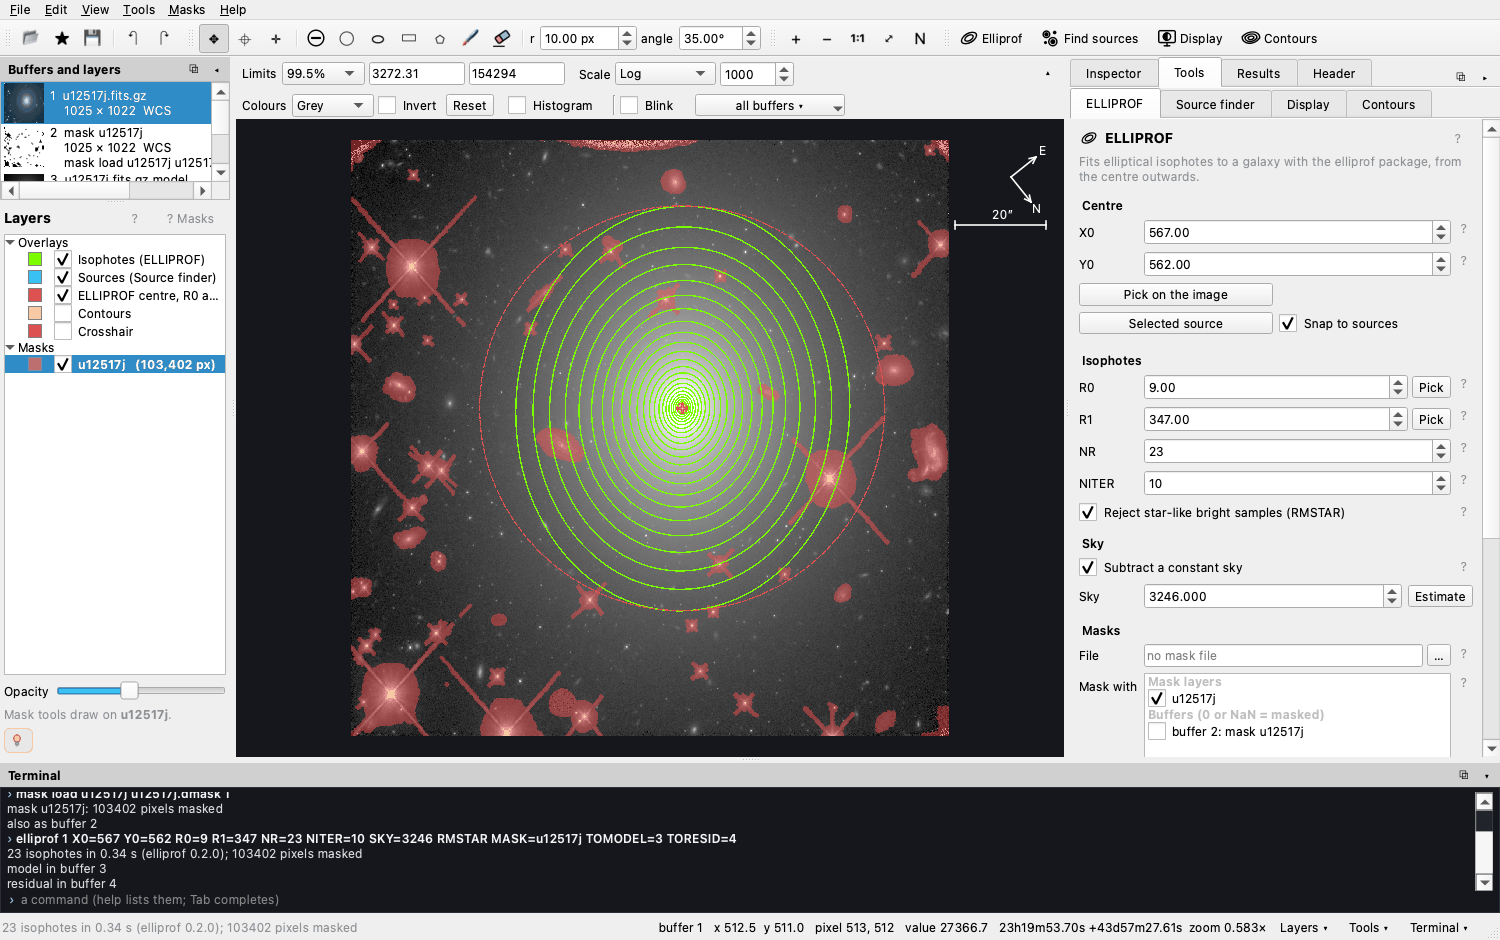
\includegraphics[width=\textwidth]{figures/hero.png}
\caption{The \avl\ window with the UGC~12517 example after an ELLIPROF fit. Left: the
image buffers and the layers (overlays and mask layers, each with its own colour). Centre:
the image, with the 23 fitted isophotes (green), the ELLIPROF centre and outer radius
(red), the published mask (red patches), the compass and the scale bar. Right: the
ELLIPROF tool, beside the Inspector, Results and Header tabs. Bottom: the terminal, which
records every command.\label{fig:window}}
\end{figure*}

\section{Design} \label{sec:design}

\avl\ is written in Python. The window uses Qt for Python \citep{pyside6} and the image
display PyQtGraph \citep{pyqtgraph}; numerical work uses NumPy \citep{Harris2020} and
SciPy \citep{Virtanen2020}, FITS input and output and world coordinates use Astropy
\citep{Astropy2013,Astropy2018,Astropy2022}, and exported figures use Matplotlib
\citep{Hunter2007}. ELLIPROF and SEP are installed as dependencies and called unchanged;
\avl\ itself contains no compiled code.

At the centre is a \emph{session} that holds numbered image buffers, mask layers,
source-finder runs and fits. The graphical interface never changes the session directly:
each button builds a command line, which is echoed in the terminal and executed by the same
interpreter that runs typed commands (Figure~\ref{fig:window}). The interface and the
command language therefore cannot disagree, and a complete session can be written out as a
plain text file and replayed with \code{astrovista --run session.txt}. Buffers remember the
command that made them, which is also written into the FITS header as a \code{HISTORY}
card when they are saved.

Three coordinate conventions coexist and are kept explicit. ELLIPROF's continuous
coordinates, in which the first pixel spans 0 to 1, are used for the fit centre, the mask
shapes and synthetic stars; integer columns and rows counted from 0 are used by pixel
statistics; and source catalogues follow SExtractor's convention, in which the centre of
the first pixel is 1. The status bar shows all of them, together with the FITS pixel index
and the sky position.

\section{Components} \label{sec:components}

\subsection{Display and inspection}

Images are recognised as FITS by their contents, whatever the file is called, and a single
image of a multi-extension file can be named by number or by \code{EXTNAME} and
\code{EXTVER} (\code{frame.fits[sci,2]}). The display offers limits from percentiles,
ZScale or the histogram; linear, logarithmic, power, square-root, asinh and
histogram-equalised stretches; twelve colour maps; contrast and bias; contours with DS9's
parameters; and an Inspector that shows the pixel under the cursor, its sky position, a
magnified view and local statistics. Blinking between buffers keeps the same patch of sky
when the images have compatible world coordinate systems, and the same pixels otherwise.

\subsection{Masks} \label{sec:masks}

Masks are layers of their own, each with a colour, an opacity and a visibility, and any
number of them can be combined in a fit. They can be drawn with circle, ellipse, box,
polygon and brush tools and an eraser. An ellipse, box or polygon waits to be applied, so
that it can first be moved, resized and rotated with handles or the keyboard
(Figure~\ref{fig:mask}); holding Alt or Shift unmasks instead, and every edit can be
undone. Masks can also be made from the data (non-finite pixels, a range of values) and,
most usefully, from the source finder: every detected source except the galaxy at the
fitting centre, enlarged by a chosen factor of its Kron ellipse \citep{Kron1980}; only the
sources that satisfy a condition on the catalogue
(\code{MAG\_AUTO < 22 and FWHM\_IMAGE < 3}); or the sources' own pixels from the
segmentation image, grown by a few pixels. When no centre has been chosen yet, the largest
detected source is assumed to be the galaxy and kept unmasked. Layers can be grown, shrunk,
inverted and combined, and are written either as FITS images or as the one-bit
\code{.dmask} bitmaps that ELLIPROF reads. In masks, 0 means masked and 1 good, as in
ELLIPROF.

\begin{figure}[t]
\centering
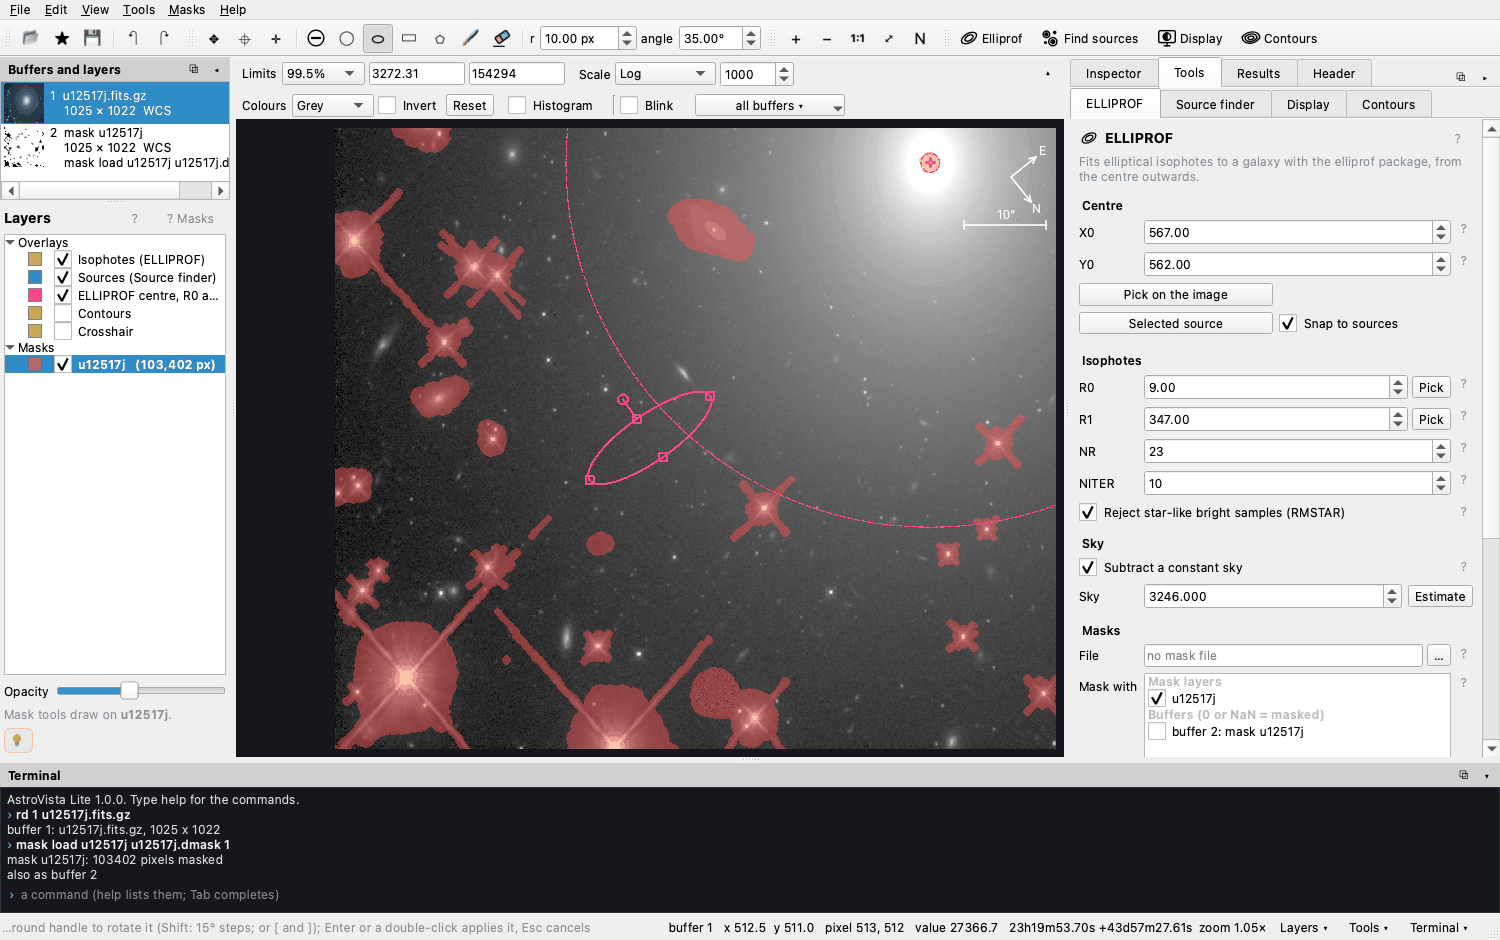
\includegraphics[width=\columnwidth]{figures/mask_rotate.png}
\caption{An elliptical mask waiting to be applied (magenta): it can be moved by dragging,
resized with its square handles and turned with the round handle (here by $35^\circ$)
before Enter applies it. The red patches are the published mask of the
example.\label{fig:mask}}
\end{figure}

\subsection{Isophote fitting}

The ELLIPROF tool collects the centre (typed, picked on the image with an optional snap
to the nearest detected source, or taken from a selected source), the first and last
semi-major axes (which can also be picked), the number of isophotes and iterations, an
optional constant sky (with a clipped-median estimate from the unmasked pixels), the
rejection of star-like samples, and the masks to use. The fit is run through elliprof; the
profile appears as a table and as plots of any column against $R$ or $R^{1/4}$, with de
Vaucouleurs' law \citep{deVaucouleurs1948} fitted on request, and the model and residual
images go into the buffers chosen. Profiles are exported as CSV files with aligned columns
or as PNG figures, and the isophotes as DS9 regions.

\subsection{Source finding}

The source finder runs SEP's background estimation, detection, deblending and photometry
with SExtractor's parameter names and defaults, and returns a catalogue with SExtractor's
columns (positions, shapes, Kron radii, half-light radii, automatic and aperture
magnitudes, flags and, when the image has a WCS, sky coordinates) together with the
segmentation image. Runs are numbered and kept, the catalogue can be sorted and plotted,
and a click on a source selects its row.

\subsection{Arithmetic and image commands}

Formulas such as \code{[3] = [1] - [2]} or \code{[4] = median([1], [2], [3])} are parsed
and evaluated pixel by pixel; they are never executed as Python. Statistics such as
\code{median([1])} reduce a single buffer to a number, and a mask layer's name stands for
1 where it is good and NaN where it masks. Division by zero, logarithms of zero and
overflows give NaN rather than infinity, and reductions ignore NaN. A set of image
commands follows the names of MONSTA: constants and buffers added, subtracted, multiplied
and divided (\code{ac}, \code{ai}, \ldots), statistics (\code{mn}, \code{abx}, \code{max}),
geometry (\code{shift}, \code{rotate}, \code{bin}, \code{mash}), smoothing and cleaning
(\code{smooth}, \code{filt}, \code{zap}, \code{clip}, \code{skysub}), synthetic stars and
noise, and FITS header editing. These are new implementations with NumPy and SciPy, with
their own options; MONSTA scripts do not run unchanged.

\subsection{The terminal}

A command line has the form \code{verb [buffer] [words] [KEY=value ...]}, with optional
quoting and comments; verbs and keywords are not case-sensitive. Variables set with
\code{set} (or by statistics commands) can stand for any keyword's value or number, so that
\code{set xc=567} followed by \code{elliprof 1 X0=xc \ldots} works as in MONSTA. Lines
that are not commands are passed to the shell when their first word is a program, which
lets users list and inspect files without leaving the window; listings are coloured and
their folders and FITS files are links. Tab completion knows commands, mask actions and
names, keywords, buffers and file names (Figure~\ref{fig:terminal}).

\begin{figure}[t]
\centering
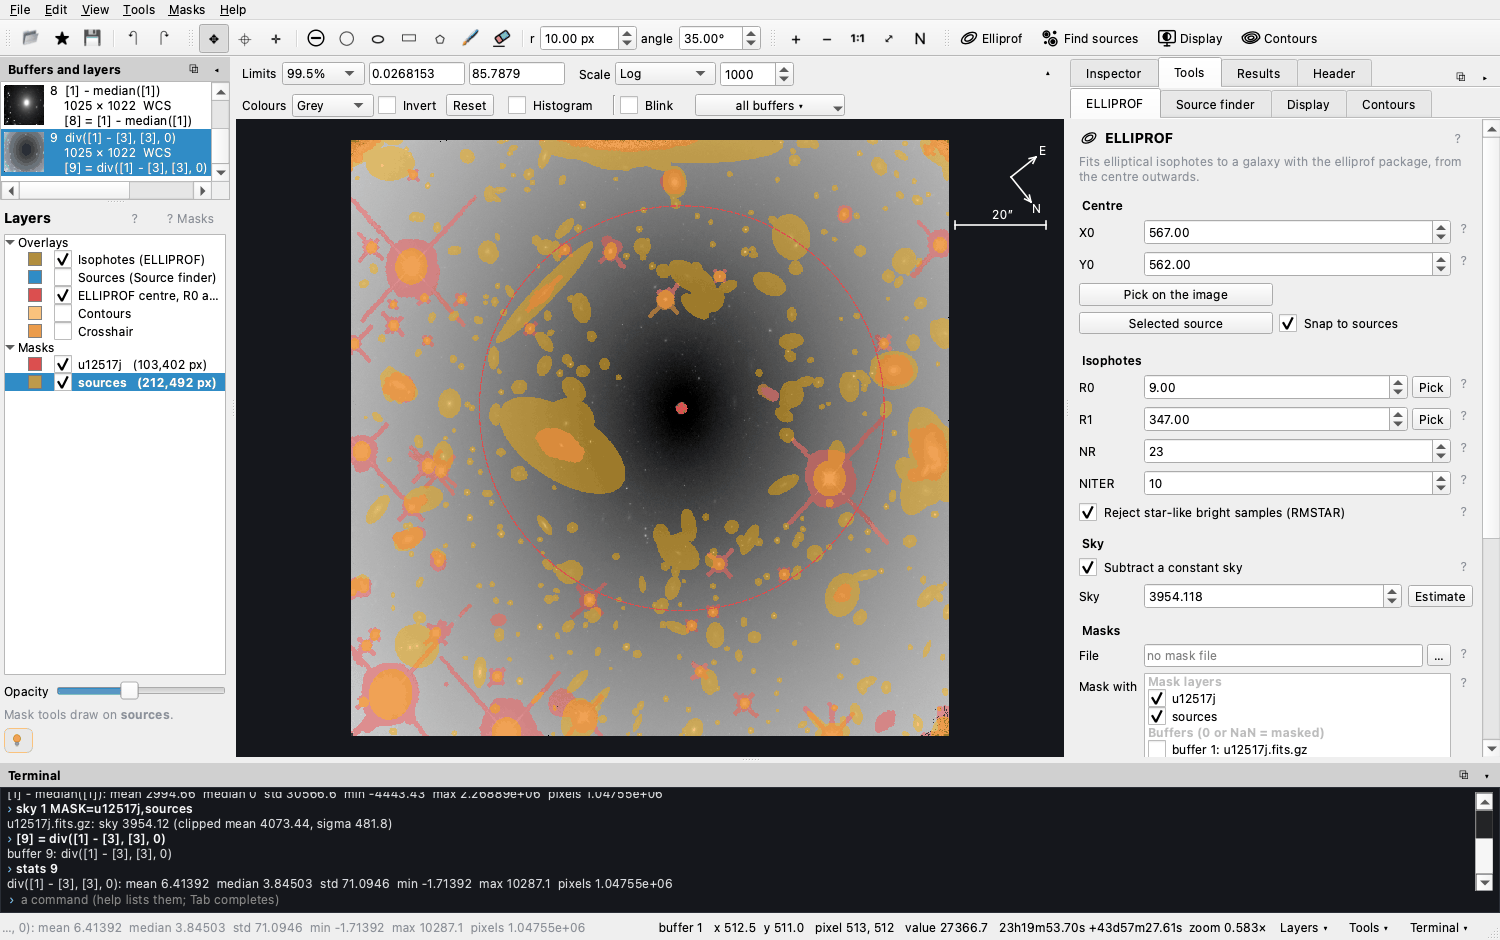
\includegraphics[width=\columnwidth]{figures/terminal.png}
\caption{Arithmetic in the terminal: the residual expressed as a fraction of the model,
\code{[9] = div([1] - [3], [3], 0)}, and its statistics. The image shows the
result.\label{fig:terminal}}
\end{figure}

\subsection{Documentation}

The documentation is part of the program. Help contains a first lesson of about thirty
minutes on the example galaxy, recipes, an account of image arithmetic, the terminal's
syntax, a reference of every command with its keywords and an example, a glossary, a FAQ
and troubleshooting, and every setting of every tool explained; the ``?'' beside each
setting opens its entry. The reference is generated from a single source that also
produces the project's web pages, and the test suite checks that every command is
documented and runs every documented example.

\section{Validation and Performance} \label{sec:validation}

We use the example shipped with the package: an HST WFC3/IR F110W image of the elliptical
galaxy UGC~12517 ($1025\times1022$ pixels of $0.128''$), with the mask of the original
analysis (103\,402 pixels, 9.9\% of the image), fitted with 23 isophotes from 9 to 347
pixels after subtracting a constant sky of 3246 counts, as in elliprof's published example.

\subsection{Agreement with elliprof}

We ran elliprof's published command-line example and the equivalent \avl\ command
(\code{elliprof 1 X0=567 Y0=562 R0=9 R1=347 NR=23 NITER=10 SKY=3246 RMSTAR MASK=u12517j}),
in which the mask is a layer loaded from the same \code{.dmask} file. The two profiles
agree in every column to the precision elliprof writes its output: the largest relative
differences are $2.6\times10^{-8}$ in intensity, $2.4\times10^{-6}$ in ellipticity,
$5.4\times10^{-6}$ in position angle and $7.8\times10^{-8}$ in the centre. The way
\avl\ prepares the image, combines masks and converts coordinates therefore leaves the
fit unchanged.

\subsection{The effect of masking the detected sources}

The source finder detects 508 sources on the image with its default settings
(Figure~\ref{fig:sources}); the stellar sequence is clearly separated at a half-light
radius of about one pixel. Masking every source except the galaxy, with Kron ellipses
enlarged by a factor of 1.5, adds 212\,492 masked pixels; together with the published mask
24.8\% of the image is excluded. Figure~\ref{fig:profiles} compares the fits with the
published mask alone and with both masks. The profiles agree closely: the outer
intensities, between 247 and 347 pixels, change by at most 1.0\%, and de Vaucouleurs' law
fitted to the whole profile gives an effective radius of 126.5 and 126.4 pixels
($16.2''$) with a scatter of 0.070 mag about the law in both cases. On the pixels left by
both masks within the last isophote, the median absolute residual is 2.6\% of the model in
both fits (Figure~\ref{fig:images}). For this galaxy the published mask already removed the
sources that matter; the source finder reproduces that result in one step and makes it
easy to check.

\begin{figure*}[t]
\centering
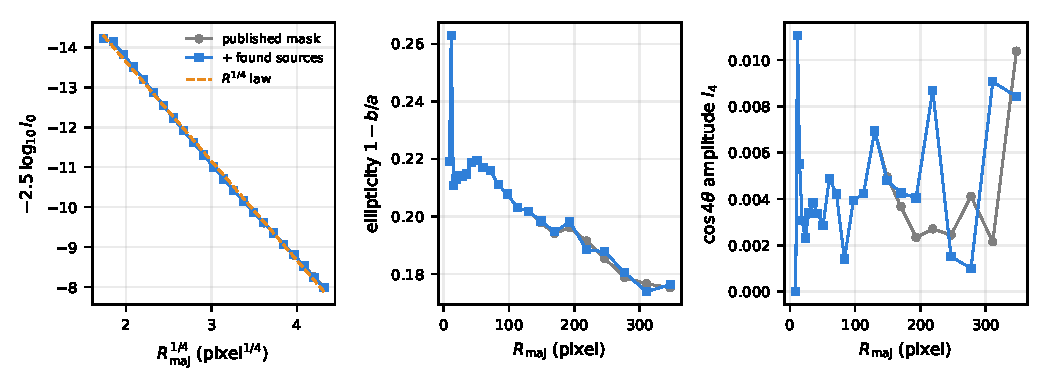
\includegraphics[width=\textwidth]{figures/profiles.pdf}
\caption{ELLIPROF profiles of UGC~12517 with the published mask (grey) and with every
detected source masked as well (blue). Left: intensity against $R_{\rm maj}^{1/4}$, with
the de Vaucouleurs law fitted to the second profile (dashed). Centre: ellipticity. Right:
amplitude of the $\cos4\theta$ term.\label{fig:profiles}}
\end{figure*}

\begin{figure*}[t]
\centering
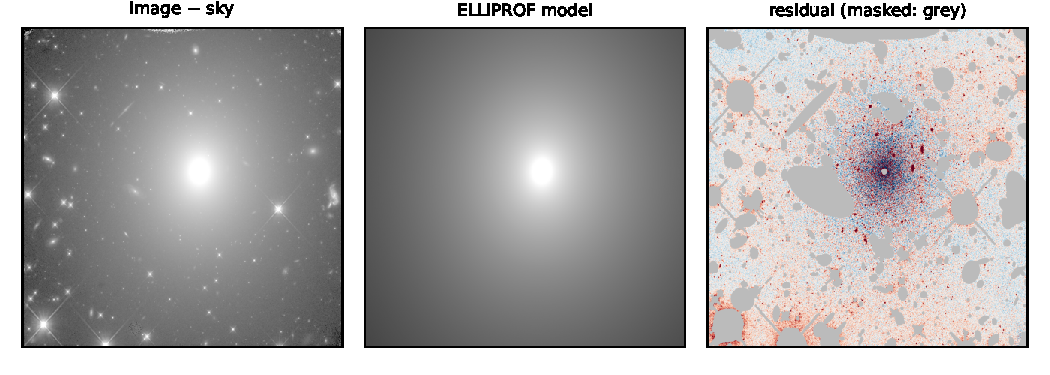
\includegraphics[width=\textwidth]{figures/images.pdf}
\caption{UGC~12517 after subtracting the sky (left), the ELLIPROF model (centre) and the
residual (right), with both masks; masked pixels are grey. The two left panels share an
asinh stretch.\label{fig:images}}
\end{figure*}

\begin{figure}[t]
\centering
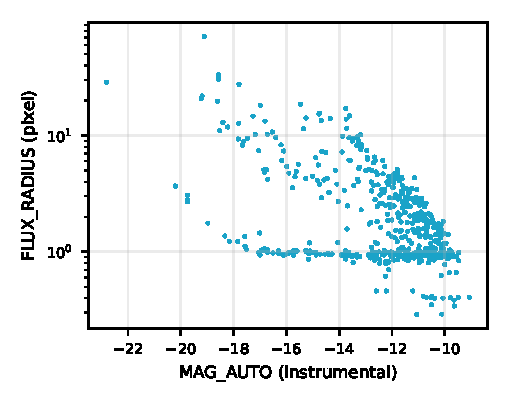
\includegraphics[width=\columnwidth]{figures/sources.pdf}
\caption{Half-light radius against instrumental magnitude for the 508 sources found on
the UGC~12517 image. Point sources form the narrow sequence near one
pixel.\label{fig:sources}}
\end{figure}

\subsection{Performance}

Table~\ref{tab:timing} lists the time taken by common commands on the example image, the
best of three runs on an Apple M5 Pro with Python 3.13. All the heavy work runs in compiled
code (ELLIPROF, SEP, NumPy and SciPy), and every command takes well under a second.
A median filter that ignores NaN pixels, which a per-pixel Python loop would take several
seconds to compute, is implemented by sorting each box with NumPy.

\begin{deluxetable}{lr}
\tablecaption{Time of common commands on the $1025\times1022$ example image.\label{tab:timing}}
\tablehead{\colhead{Command} & \colhead{Time (s)}}
\startdata
Read the image (FITS) & 0.002 \\
ELLIPROF, 23 isophotes, model and residual & 0.10 \\
Source finder (508 sources) & 0.11 \\
\code{[5] = [1] - median([1])} & 0.008 \\
Median of three images & 0.06 \\
Gaussian smoothing, FWHM 3 pixels & 0.014 \\
Median filter $5\times5$, NaN pixels ignored & 0.19 \\
Cosmic-ray cleaning (\code{zap}) & 0.46 \\
Rotation by $12.5^\circ$ & 0.04 \\
\enddata
\tablecomments{Measured with \code{paper/make\_figures.py} in the repository.}
\end{deluxetable}

\subsection{Testing}

The test suite contains 65 tests that run without a display, covering the commands,
masks and their undo history, arithmetic and its special values, the source finder, the
fit, the window's tools and panels, and the documentation; one test runs every example
shown on the project's web pages, in order, on the example image. Continuous integration
runs the suite on Ubuntu (x86\_64 and ARM) and macOS with Python 3.10 to 3.13, and runs a
complete session in a real X11 window on Linux.

\section{Use in Teaching} \label{sec:teaching}

The program opens on a welcome screen that offers the example, an image of the user's own
or the first lesson. The lesson takes about thirty minutes and walks through a complete
measurement: looking at the light with different stretches, finding and classifying the
sources, choosing the centre and radii, masking, fitting, reading the profile and its
$R^{1/4}$ law, and studying the residual, with a question at each step. Because every step
is echoed as a command, students see the language as they work, and a teacher can hand out
a command file so that every student starts from the same place. Making masks, a slow
part of fitting real galaxies, becomes a short exercise, and the \code{.dmask} files
students produce can be used directly with elliprof.

\section{Availability} \label{sec:availability}

\avl\ is released under the MIT licence at \url{https://github.com/ekourkchi/AstroVista-Lite}
and on the Python Package Index as \code{AstroVista}. It requires Python 3.10 or later and
runs on macOS 13 or later and on Linux with glibc 2.34 or later; a conda environment
provides it on older systems. The website \url{https://ekourkchi.github.io/AstroVista-Lite/}
has a tutorial, the terminal guide and the command reference. The figures and numbers of
this paper are produced by \code{paper/make\_figures.py} in the repository.

\section{Summary} \label{sec:summary}

\avl\ gathers the steps of an isophote fit (display, source finding, masking, fitting and
inspection) into one window built around a reproducible command language that follows
MONSTA. It reproduces elliprof's published fit exactly, makes masks for ELLIPROF quickly,
and documents itself for students. Future work in the full AstroVista includes further
measurements, multiple linked views and regions.

\begin{acknowledgments}
ELLIPROF and the MONSTA command language are the work of John Tonry; MONSTA joined Vista,
originally by Richard Stover and Tod Lauer with image display by John Tonry, and Mongo, by
John Tonry. The source finder uses SEP by Kyle Barbary and contributors. The example image
of UGC~12517 comes from the elliprof package's example.
%% TODO (to be completed by the author): an account of the generative AI assistance,
%% consistent with the JOSS paper's disclosure (tools and versions, where they were used,
%% and that the author reviewed, edited and validated all of it).
\textbf{[AI assistance statement to be added by the author.]}
\end{acknowledgments}

\software{elliprof \citep{elliprof}, SEP \citep{Barbary2016}, Astropy
\citep{Astropy2013,Astropy2018,Astropy2022}, NumPy \citep{Harris2020}, SciPy
\citep{Virtanen2020}, Matplotlib \citep{Hunter2007}, PyQtGraph \citep{pyqtgraph}, Qt for
Python \citep{pyside6}}

\bibliography{paper}{}
\bibliographystyle{aasjournalv7}

\end{document}
